
\begin{example}
Sea $W$ el sólido limitado por el cilindro parabólico $y = x^2$ y los planos $z = 0$, $z = 4$ y $y = 1$. Calcular $\iiint_W yz \: dV$. 
\end{example}


\textbf{Soluci\'on:}
\begin{figure}[htbp]
    \centering
    % Llamamos al archivo con el código TikZ extraído
    \begin{center}
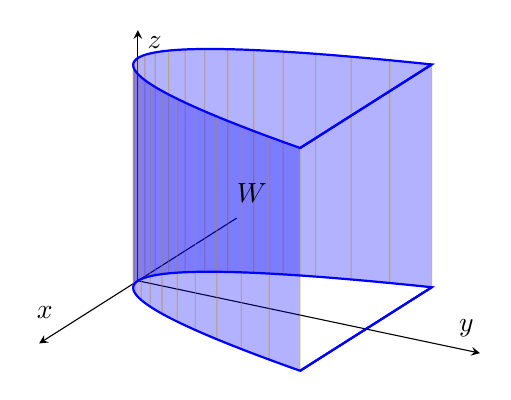
\begin{tikzpicture}
    \begin{axis}[
        view={120}{30},
        axis lines=center,
        xlabel=$x$, ylabel=$y$, zlabel=$z$,
        xmin=-1.5, xmax=1.5, ymin=0, ymax=1.5, zmin=0, zmax=4.5,
        ticks=none,
        clip=false
    ]
        % Superficie lateral y=x^2
        \addplot3[surf, opacity=0.3, blue, domain=-1:1, y domain=0:4, samples=25, samples y=2] (x, {x^2}, y);
        
        % Líneas de contorno para dar definición
        \addplot3[thick, blue, domain=-1:1, samples=50] (x, {x^2}, 0);
        \addplot3[thick, blue, domain=-1:1, samples=50] (x, {x^2}, 4);
        \draw[thick, blue] (axis cs:-1,1,0) -- (axis cs:1,1,0);
        \draw[thick, blue] (axis cs:-1,1,4) -- (axis cs:1,1,4);
        
        \node at (axis cs:0,0.5,2) {$W$};
    \end{axis}
\end{tikzpicture}
\end{center} 
    \label{fig:ejemplo 8.2.2}
\end{figure}

La región $W$ puede describirse como:
\[
    W = \{ (x,y,z) \in \Rn{3} : -1 \leq x \leq 1; \; x^2 \leq y \leq 1; \; 0 \leq z \leq 4 \}.
\]
Aplicando el Teorema de Fubini:
\begin{gather*}
    \iiint_W yz \: dV = \int_{-1}^{1} \int_{x^2}^{1} \int_{0}^{4} yz \: dz \, dy \, dx = \int_{-1}^{1} \int_{x^2}^{1} y \left[ \frac{z^2}{2} \right]_0^4 dy \, dx \\
    = \int_{-1}^{1} \int_{x^2}^{1} 8y \: dy \, dx = 8 \int_{-1}^{1} \left[ \frac{y^2}{2} \right]_{x^2}^1 dx = 4 \int_{-1}^{1} (1 - x^4) \: dx \\
    = 4 \left[ x - \frac{x^5}{5} \right]_{-1}^1 = 4 \left( \left( 1 - \frac{1}{5} \right) - \left( -1 + \frac{1}{5} \right) \right) = 4 \left( \frac{4}{5} + \frac{4}{5} \right) = \frac{32}{5}.
\end{gather*}


\clearpage

\begin{example}  Hallar el volumen del cuerpo $W$  dentro de la esfera  \(x^2+y^2+z^2=32\)  tal que
\(z \geq \sqrt{x^2+y^2}\).
\end{example}

\begin{figure}[htbp]
    \centering
    % Llamamos al archivo con el código TikZ extraído
    \begin{figure}[H]
    \centering
    \tikzsetnextfilename{ejercicio30_figura} 

    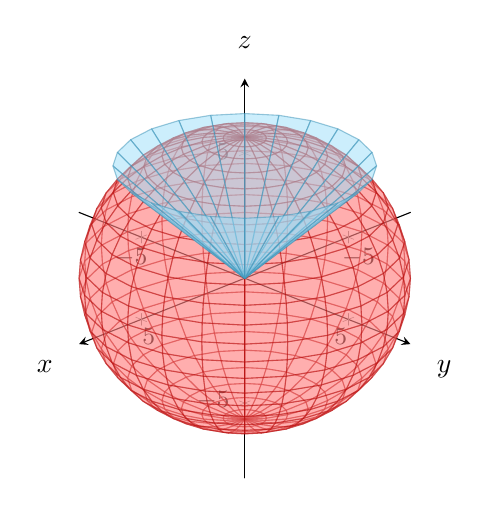
\begin{tikzpicture}[line cap=round, line join=round]
        \begin{axis}[
            view={135}{25}, % Cámara clásica
            width=10cm,
            height=10cm,
            axis lines=center,
            % 1. Ajustamos los ejes al nuevo tamaño de la esfera (aprox 5.65)
            xmin=-8, xmax=8, 
            ymin=-8, ymax=8,
            zmin=-8, zmax=8,
            xlabel={$x$},
            ylabel={$y$},
            zlabel={$z$},
            every axis x label/.style={at={(ticklabel* cs:1.05)},anchor=north east},
            every axis y label/.style={at={(ticklabel* cs:1.05)},anchor=north west},
            every axis z label/.style={at={(ticklabel* cs:1.05)},anchor=south},
            ticklabel style={font=\small},
        ]

        % Esfera de radio \sqrt{32} (Roja transparente)
        \addplot3[
            surf,
            opacity=0.4,
            color=red!50,
            faceted color=red!70!black,
            samples=25, 
            domain=0:360,
            y domain=0:180,
            z buffer=sort
        ]
        ({sqrt(32)*cos(x)*sin(y)}, {sqrt(32)*sin(x)*sin(y)}, {sqrt(32)*cos(y)});

        % Cono Superior z = \sqrt{x^2+y^2} (Celeste transparente)
        \addplot3[
            surf,
            opacity=0.5,
            color=cyan!40,
            faceted color=cyan!70!black,
            samples=25,
            samples y=2, 
            domain=0:360,
            % 2. El cono se interseca en z=4. Le damos hasta 4.5 para que lo atraviese bien
            y domain=0:4.5, 
            z buffer=sort
        ]
        ({y*cos(x)}, {y*sin(x)}, {y});

        \end{axis}
    \end{tikzpicture}
    \caption{Representación de la región pedida. \href{https://www.geogebra.org/m/pvzc3wke}{Ver en GeoGebra}}
    \label{fig:ejercicio30_figura}
\end{figure} 
    \label{fig:Ejemplo 8.2.3}
\end{figure}


\textbf{Soluci\'on:} La superficies $x^2+y^2+z^2=32$  y  $z=\sqrt{x^2+y^2}$ son,  una esfera de radio \(R=4\sqrt{2}\)    y un semicono superior, respectivamente, como se muestra en la figura~\ref{fig:ejercicio30_figura}. 


Plantearemos  la soluci\'on del problema con distintos cambios de cooredenadas. 



La intersección entre  ambas superficies se obtiene de
\[
r=z, \quad r^2+z^2=32 \Rightarrow 2r^2=32 \Rightarrow r=4.
\]

\textbf{1. Coordenadas cartesianas:} El s\'olido  $W$ cumple que
\[
x^2+y^2+z^2 \le 32, \quad z \ge \sqrt{x^2+y^2},
\] podemos describirlo por
\[
W=\left\{(x,y,z):
-4  \le x\le 4,\;
-\sqrt{16-x^2}\le y\le \sqrt{16-x^2},\;
\sqrt{x^2+y^2}\le z\le \sqrt{32-x^2-y^2}
\right\}
\]luego,  \[
Vol (W)=\int_{-4}^{4}
\int_{-\sqrt{16-x^2}}^{\sqrt{16-x^2}}
\int_{\sqrt{x^2+y^2}}^{\sqrt{32-x^2-y^2}}
dz\,dy\,dx.
\]

\bigskip

\textbf{2. Coordenadas cilíndricas:} Usando la transformación en coordenadas cilíndricas (~\ref{def:coord_cilindricas}), el s\'olido $W$ podemos describirlo por
\[
W=\left\{(r,\theta,z):
0 \le \theta \le 2\pi,\;
0 \le r \le 4,\;
r \le z \le \sqrt{32-r^2}
\right\}
\]luego,
\[
Vol (W)=\int_{0}^{2\pi}
\int_{0}^{4}
\int_{r}^{\sqrt{32-r^2}}
r \, dz\,dr\,d\theta.
\]

\bigskip


\textbf{3. Coordenadas esféricas:} Usando la transformación en coordenadas esféricas (~\ref{def:coord_esfericas}), el s\'olido $W$ podemos describirlo por
\[
W=\left\{(\rho,\theta,\varphi):
0 \le \theta \le 2\pi,\;
0 \le \varphi \le \frac{\pi}{4},\;
0 \le \rho \le 4\sqrt{2}
\right\}
\]luego,
\[
Vol (W)=\int_{0}^{2\pi}
\int_{0}^{\pi/4}
\int_{0}^{4\sqrt{2}}
\rho^2\sin\varphi \, d\rho\,d\varphi\,d\theta.
\]

\bigskip
Calculando la integral triple en coordenadas esféricas:
\[
Vol(W) = \int_{0}^{2\pi} d\theta \cdot \int_{0}^{\pi/4} \sin\varphi \, d\varphi \cdot \int_{0}^{4\sqrt{2}} \rho^2 \, d\rho.
\]
Resolviendo cada integral iterada de forma independiente:
\[
\int_{0}^{2\pi} d\theta = 2\pi,
\]
\[
\int_{0}^{\pi/4} \sin\varphi \, d\varphi = \Big[ -\cos\varphi \Big]_{0}^{\pi/4} = -\frac{\sqrt{2}}{2} - (-1) = 1 - \frac{\sqrt{2}}{2},
\]
\[
\int_{0}^{4\sqrt{2}} \rho^2 \, d\rho = \left[ \frac{\rho^3}{3} \right]_{0}^{4\sqrt{2}} = \frac{(4\sqrt{2})^3}{3} = \frac{128\sqrt{2}}{3}.
\]
Multiplicando los tres resultados:
\[
Vol(W) = 2\pi \cdot \left(1 - \frac{\sqrt{2}}{2}\right) \cdot \frac{128\sqrt{2}}{3} = \frac{256\sqrt{2}\pi}{3} \left(1 - \frac{\sqrt{2}}{2}\right) = \frac{256\pi}{3}(\sqrt{2}-1).
\]

\[
\boxed{Vol(W) = \frac{256\pi}{3}(\sqrt{2}-1)}
\]